\appendix
% \appendixpage
% \addappheadtotoc
\newcommand{\norm}[1]{\left\lVert#1\right\rVert}

\chapter[Regiones \Ion{H}{II}]{Regiones \boldmath{\Ion{H}{II}} \citep{Stahler:2004}}
\label{app:HII}

%\newcommand\N{\ensuremath{\mathcal{N}}}

Consideremos el caso en que se forma una estrella masiva dentro de una nube molecular, que por simplicidad está compuesta exclusivamente de hidrógeno molecular $\mathrm{H_2}$. La estrella masiva emite fotones ultravioleta que tienen la energía suficiente para disociar el $\mathrm{H_2}$  como para ionizar el hidrógeno atómico resultante. Luego el plasma ionizado se recombina para volver a ser \Ion{H}{I} emitiendo líneas espectrales de diversas energías, siendo la más energética la línea de \Ion{Ly}{\alpha}. Como al realizar una ionización se pierde un fotón ionizante y el flujo de radiación proveniente de la estrella es finito, entonces la estrella solo puede ionizar la región de la nube más próxima a ésta. Si suponemos que la nube tiene densidad uniforme, entonces esta región tendrá forma esférica, conocida como \textit{esfera de Strömgren}.

\section{Esfera de Strömgren}

El plasma ionizado dentro de la Esfera de Strömgren se encuentra en balance de ionización, esto es, que la tasas de ionización y la de recombinación son iguales. La tasa de ionizaciones es igual a la cantidad de fotones ionizantes que emite la estrella central por segundo. Esto es, los fotones que poseen una energía mayor al límite de Lymann, que corresponde a  $E = \SI{13.6}{eV}$, o bien $\lambda = \SI{912}{\angstrom}$. En la tabla \ref{tab:ionizing-radiation} se muestra la tasa de fotones ionizantes $\Nio_*$ para estrellas masivas de tipo espectral O y B temprano.

\begin{table}
  \centering
  \begin{tabular}{cccc} \toprule
    Tipo & Masa & $\log \Nio_*$ & $\log \Nio_{FUV}$ \\
    Espectral & (\SI{}{M_\odot}) & (\SI{}{s^{-1}}) & (\SI{}{s^{-1}})  \\
    \midrule
    O4 & 70 & 49.9 & 49.5 \\
    O5 & 60 & 49.4 & 49.2 \\
    O6 & 40 & 48.8 & 48.8 \\
    O7 & 30 & 48.5 & 48.6 \\
    O8 & 23 & 48.2 & 48.4 \\
    O9 & 20 & 47.8 & 48.2 \\
    B0 & 18 & 47.1 & 48.1 \\
    B1 & 13 & 45.4 & 47.5 \\
    B2 & 10 & 44.8 & 47.1 \\
    \bottomrule
  \end{tabular}
  \caption{Tasa de fotones ionizantes para estrellas masivas \citep{Stahler:2004}}
  \label{tab:ionizing-radiation}
\end{table}

El radio de esta esfera se denomina \textit{Radio de Strömgren} que viene dado por:


\begin{align}
  R_s = \left[\frac{3\Nio_*}{4\pi\alpha'_{rec}(n^0_H)^2}\right]^{1/3} = 0.4\mathrm{~pc}\left(\frac{\Nio_*}{10^{49}\mathrm{~s^{-1}}}\right)^{1/3}\left(n_{H_2}\right)^{-2/3} \label{eq:stromgren}
\end{align}

Donde $\alpha'_{rec}$ es el coeficiente de recombinación a todos los niveles energéticos del hidrógeno excepto el estado base, $n^0_H$ y $n_{H_2}$ son la densidad numérica del hidrógeno neutro y del hidrógeno molecular donde está embebida la región HII, respectivamente.

En la expresión numérica, se adopta una temperatura de $10^4\mathrm{~K}$ que es la temperatura característica de una región \Ion{H}{II} y con la que el coeficiente de recombinación $\alpha'_{rec}$ adopta un valor de \SI{2.6e-13}{cm^3.s^{-1}}.

Dentro de la región \Ion{H}{II}, la probabilidad por unidad de tiempo de ionizar un átomo de hidrógeno dado es mucho mayor a la probabilidad de una recombinación, por lo que el gas está casi completamente ionizado. Sin embargo, en los bordes la densidad de gas neutro aumenta debido a que en dicha región el flujo de fotones ionizantes ha sido atenuado por todo el gas ionizado más próximo a la estrella. La transición de gas ionizado a gas neutro tiene un grosor $\Delta r$ que corresponde al camino libre medio del gas neutro. Esto es:

\begin{align}
\Delta R = \frac{1}{\sigma_{\nu_1}n^0_H}  
\end{align}

Donde $\sigma_{\nu_1}$ es la sección recta de un átomo de hidrógeno en el estado base, evaluada en la longitud de onda del límite de Lymann. Utilizando $\sigma_{\nu_1} = \SI{6.8e-18}{cm^2}$ y $n^0_H = \SI{2e3} 10^{3}{cm^{-3}}$ obtenemos que $\Delta r = \SI{7.4e13}{cm} \sim \SI{5e-5}{R_s}$, lo que muestra que las regiones \Ion{H}{II} tienden a tener bordes bien delimitados.

Sin embargo, las esferas de Strömgren no son objetos estáticos, sino que se expanden con el tiempo. Este proceso ocurre en dos etapas: en la primera inicialmente no existe ninguna región \Ion{H}{II} pero que la radiación ultravioleta de la estrella hace que se expanda de manera exponencial al disociar e ionizar el gas a su alrededor hasta alcanzar el radio de Strömgren. Posteriormente la diferencia de presiones entre el gas ionizado de la región \Ion{H}{II} y del gas neutro circundante, provoca una segunda expansión con forma de ley de potencias hasta alcanzar equilibrio de presiones.

\section{Flujos de Champaña}
La segunda expansión lleva a que la región \Ion{H}{II} se expanda dos órdenes de magnitud por encima del radio de Strömgren, pero el tiempo que toma alcanzar dichas dimensiones es tan largo que la estrella central muere antes de se alcanze el equilibrio de presiones. Sin embargo, es más probable que el frente de ionización rebase el borde de la nube molecular donde se formó, y en este caso el gas ionizado altamente presurizado escapa directamente hacia el medio interestelar que lo rodea (que tiene una presión aún menor que la de la nube molecular), creando el \textit{Flujo de champaña}.

\section{Características de la emisión}

Tradicionalmente la línea de \Ion{H}{\alpha} es la que se utiliza para detectar regiones \Ion{H}{II} en el óptico, sin embargo, otras líneas espectrales, tales como iones de carbono, oxígeno y nitrógeno también son importantes. Es más, aunque estos iones son relativamente poco abundantes, poseen estados meta-estables que pueden ser excitados por electrones del ambiente que tengan solo unos pocos eV de energía, y posteriormente emitir líneas prohibidas de emisión. La sección transversal para la excitación de la línea es relativamente grande, aun más que la de la recombinación electrón-protón, por lo que la emisión de líneas prohibidas es un proceso de enfriamiento más eficaz que la recombinación en cascada del hidrógeno. Los iones más comunes de estos metales son los que están ionizados varias veces, tales como el [\Ion{O}{II}], que emite en óptico el doblete $\lambda\lambda 3726-\SI{3729}{\angstrom}$, el [\Ion{O}{III}], que emite en óptico el doblete $\lambda\lambda 4959-\SI{5007}{\angstrom}$, el [\Ion{N}{II}] que tiene dos transiciones que emiten a las longitudes de onda de $\lambda \SI{6583}{\angstrom}$ y $\lambda \SI{6548}{\angstrom}}$, y el [\Ion{C}{IV}] a $\lambda \SI{1549}{\angstrom}$ en ultravioleta.
Por otro lado, en radio continuo observamos radiación libre-libre. A bajas frecuencias, donde la aproximación de Rayleigh-Jeans es válida, el coeficiente de absorción es proporcional a $\nu^{-2}$. Por tanto, a bajas frecuencias la región \Ion{H}{II} es ópticamente gruesa respecto a frecuencias más altas. En el régimen ópticamente grueso, la emisividad es proporcional a $\nu^{2}$ y la pendiente nos da una estimación directa de la temperatura. Por otro lado, en el régimen ópticamente delgado, el flujo es proporcional a la medida de emisión, por lo que teniendo la región \Ion{H}{II} espacialmente resuelta, podemos tener una estimación de la densidad electrónica.

%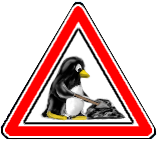
\includegraphics[width=0.1\linewidth]{./Figures/tux-development}

\chapter{Choques y Frentes de Ionización}
\label{app:shocks}
\thispagestyle{empty}
Algunas veces en un medio gaseoso pueden existir discontinuidades importantes en alguna de sus propiedades físicas, cuando estas propiedades son la presión, densidad y temperatura del gas nos estamos refiriendo a un choque, que es producido cuando el gas sufre una perturbación a una velocidad superior a la del sonido, mientras que si la discontinuidad ocurre en el grado de ionización del gas, entonces esta discontinuidad es conocida como frente de ionización. En esta sección analizaremos las condiciones de salto tanto de los choques como de los frentes de ionización para conocer las propiedades del gas en las dos interfaces de la discontinuidad.
\section{Choques}

Consideremos un fluído que tiene densidad $\rho_1$, presión $P_1$ y se mueve en la dirección de eje $+x$ con velocidad $u_1$. En la posición $x = s(t)$ existe un choque que se mueve a velocidad $u_0\equiv \frac{ds}{dt}$. Delante del choque el fluído tiene densidad $\rho_2$, presión $P_2$ y se mueve a velocidad $u_2$.

Antes y después del choque escogemos dos puntos arbitrarios, $x_1$ y $x_2$, respectivamente que forman una superficie cada uno en el plano $yz$ que están en co-movimiento con la discontinuidad (ver figura \ref{fig:shock}). 

\begin{figure}
  \centering
  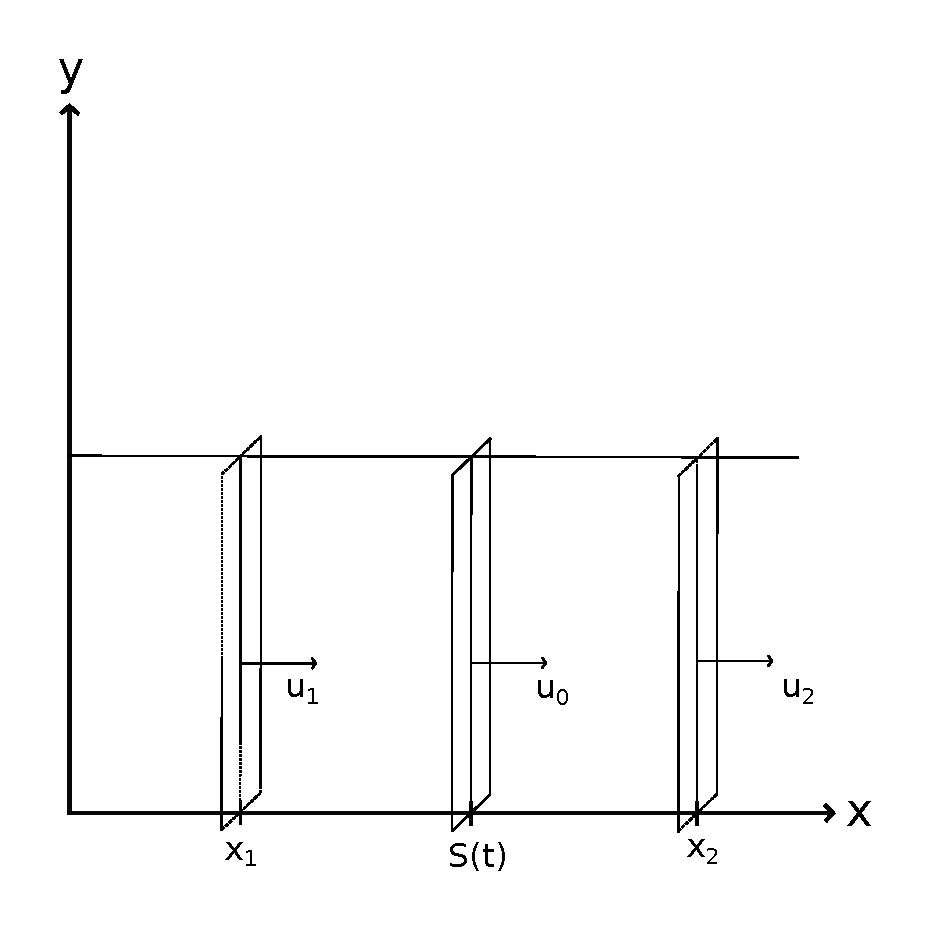
\includegraphics[width=0.7\linewidth]{./Figures/shock}
  \caption{Representación esquemática de un fluido con una discontinuidad situada en $x=s(t)$. Detrás y delante del choque en las posiciones $x=x_1$ y $x=x_2$, respectivamente, situamos dos superficies paralelas al choque y que están en co-movimiento con éste.}
  \label{fig:shock}
\end{figure}

La masa encerrada dentro del volumen que forman las dos superficies es constante en el tiempo, esto es, la cantidad que fluido que entra por la superficie 1 (atrás del choque), debe ser igual a la que sale por la superficie 2:

\begin{align}
  \frac{d}{dt}\int^{x_2}_{x_1} \rho~dx = 0 \label{eq:rho-dx}
\end{align}

Por otro lado, dentro del volumen entre las dos superficies, la presión del fluído en la superficie 1 contribuye a incrementar el momento, mientras que la presión en la superficie 2 tiene el efecto contrario, entonces:

\begin{align}
  \frac{d}{dt}\int^{x_2}_{x_1} \rho u~dx = P_1 - P_2 \label{eq:u-rho-dx}
\end{align}

Por último, por completez la potencia mecánica por unidad de área $P_1u_1 - P_2u_2$ incrementa la energía interna del fluído entre las superficies:

\begin{align}
  \frac{d}{dt}\int^{x_2}_{x_1} \rho\left(\frac{u^2}{2} + \epsilon\right)~dx = P_1u_1 - P_2u_2 \label{eq:rho-u2-epsilon-dx}
\end{align}

Donde $\epsilon$ es la energía interna por unidad de masa. Nótese que esta ecuación no es válida si el fluído puede perder energía por radiación (este caso se discutirá aparte más adelante).

Las tres ecuaciones anteriores son de la siguiente forma:

\begin{align}
  \frac{dJ}{dt} \equiv \frac{d}{dt}\int^{x_2}_{x_1} \Psi(x, t)~dx
\end{align}

Donde $\Psi(x, t)$ presenta una discontinuidad espacial en $x=s(t)$. Como la integral implica solo la coordenada espacial y la derivada es respecto al tiempo, entonces podemos intercambiar el orden de éstas:

\begin{align}
    \frac{dJ}{dt} = \int^{x_2}_{x_1} \frac{d\Psi}{dt}~dx = \int^{x_2}_{x_1} \left(\frac{\partial\Psi}{\partial t} + \frac{\partial\psi}{\partial x}\frac{dx}{dt}\right)~dx
\end{align}

Debido a la discontinuidad separaramos el segundo término de la integral:

\begin{align}
  \begin{split}
    \frac{dJ}{dt} = \int^{x_2}_{x_1} \frac{\partial\Psi}{\partial t}~dx + \int^{s}_{x_1}\frac{\partial\psi}{\partial x}\frac{dx}{dt}~dx +  \int^{x_2}_{s}\frac{\partial\psi}{\partial x}\frac{dx}{dt}~dx \\= \int^{x_2}_{x_1}\frac{\partial\Psi}{\partial t}~dx\left(\Psi_1u_0-\Psi_1u_1+\Psi_2u_2-\Psi_2u_0\right) \label{eq:dj-dt}
    \end{split}
\end{align}

Como $x_1$ y $x_2$ son puntos arbitrarios, podemos tomar el límite cuando $x_1, x_2 \to s$. Este límite es de interés ya que los choques en muchos casos son muy delgados en comparación con el tamaño característico del sistema. De esta manera el primer término del lado derecho de la ecuación (\ref{eq:dj-dt}) desaparece porque la derivada parcial respecto al tiempo de $\Psi$ es finita para toda $x$ (incluída la discontinuidad). Entonces:

\begin{align}
  \lim_{x_1, x_2 \to s}\frac{dJ}{dt} = \Psi_2v_2 - \Psi_1v_1 \label{eq:dj-dt-lim}
\end{align}
Donde $v_2\equiv u_2 - u_0$ y $v_1 \equiv u_1-u_0$ son las velocidades del fluído respecto a la velocidad del choque.

Utilizando la ecuación (\ref{eq:dj-dt-lim}) en (\ref{eq:rho-dx}) obtenemos la primera condición de salto:

\begin{align}
  \rho_1v_1 = \rho_2v_2 \label{eq:jump-1}
\end{align}

Aplicando a su vez en la ecuación (\ref{eq:u-rho-dx}) con ayuda de la ecuación (\ref{eq:jump-1}) obtenemos la siguiente condición de salto:

\begin{align}
  \rho_1v^2_1 = \rho_2v^2_2 \label{eq:jump-2}
\end{align}

Por último, la última condición de salto, solo válida para sistemas adiabáticos es, utilizando la ecuación (\ref{eq:rho-u2-epsilon-dx}) es:

\begin{align}
  \frac{1}{2}v^2_1 + \epsilon_1 + \frac{P_1}{\rho_1} = \frac{1}{2}v^2_2 + \epsilon_2 + \frac{P_2}{\rho_2} \label{eq:jump-3}
\end{align}

Para el caso en que el fluído pierde energía por radiación, la ecuación (\ref{eq:u-rho-dx}) sufre la siguiente modificación:

\begin{align}
     \frac{d}{dt}\int^{x_3}_{x_1} \rho\left(\frac{u^2}{2} + \epsilon\right)~dx = P_1u_1 - P_3u_3 -2F_{rad}\label{eq:rho-u2-epsilon-dx-rad}
\end{align}

Donde $F_{rad}$ es el flujo de radiado por el fluído y $x_3$ es un punto localizado más allá de la región de relajamiento del choque (la zona donde el fluído está radiando, como referencia podemos tomar la figura 3 de \citet{Shull:1979}).

De esta forma, la nueva condición de salto en caso de un choque radiativo es:

\begin{align}
  \frac{1}{2}v^2_3 + \epsilon_3 + \frac{P_3}{\rho_3} = \frac{1}{2}v^2_1 + \epsilon_1 + \frac{P_1}{\rho_1} \frac{2F_{rad}}{\rho_1v_1}\label{eq:jump-rad}
\end{align}


\section{Frentes de Ionización}
Para esta sección, utilizaremos el subíndice ``0'' para las propiedades del gas en la interfaz neutra, mientras que para la interfaz ionizada utilizaremos el subídice ``i'' (ver figura \ref{fig:IF}). Bajo esta nomenclatura, combinando las ecuaciones (\ref{eq:jump-1}, \ref{eq:jump-2}) para las condiciones de salto en el Frente de ionización y reescribiendo la presión en términos de la velocidad del sonido:

\begin{figure*}
  \centering
  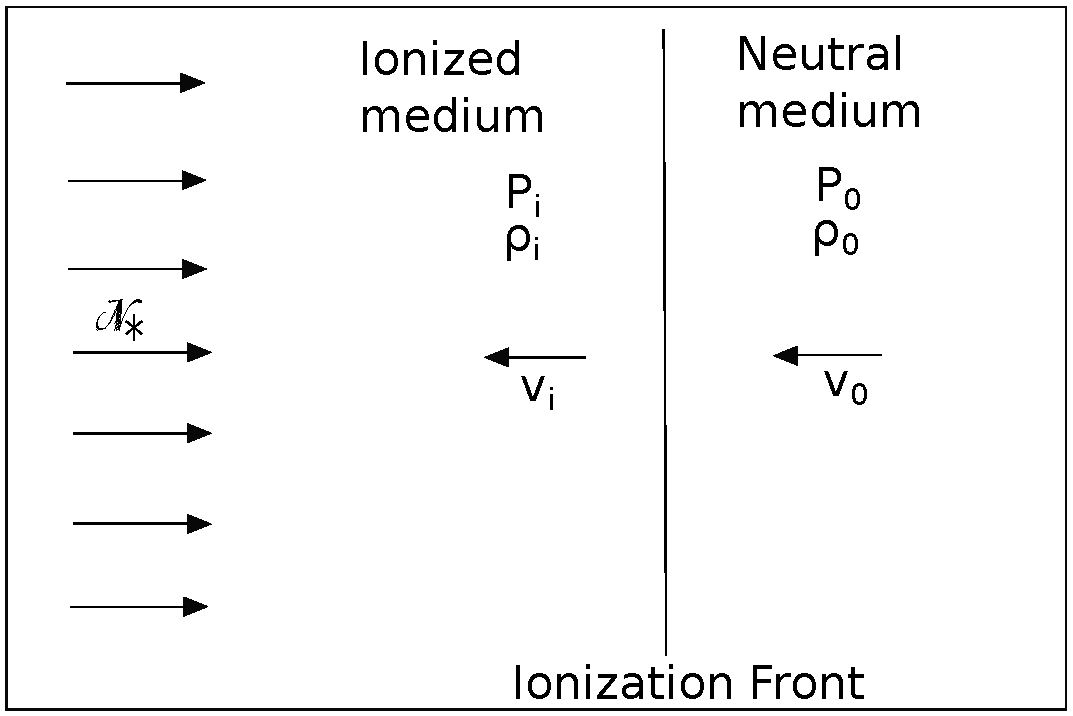
\includegraphics[width=0.8\linewidth]{./Figures/IF}
  \caption{Representación esquemática de la estuctura de un frente de ionización. En un medio gaseoso, con densidad $\rho_0$, presión $P_0$ y que se mueve velocidad $v_1$ está expuesto a radiación ionizante con flujo $\Nio_*$. El gas ionizado tiene densidad $\rho_i$, presión $P_i$ y se mueve a velocidad $v_i$. Las velocidades están medidas en el sistema de referencia del frente de ionización.}
  \label{fig:IF}
\end{figure*}

\begin{align}
  P_x = c^2_x\rho_x
\end{align}

Donde el subíndice ``x'' puede hacer referencia tanto al medio neutro o ionizado, encontramos el salto en densidad del frente de ionización:

\begin{align}
  \frac{\rho_i}{\rho_0} = \frac{1}{2c^2_i}\left[v^2_0 + c^2_0 \pm \left(\left(v^2_0 + c^2_0\right)^2 -4v^2_0c^2_i\right)^{1/2}\right]
\end{align}
O bien, en términos del número de Mach del gas neutro $\mathcal{M}\equiv v_0/c_0$:

\begin{align}
    \frac{\rho_i}{\rho_0} = \frac{1}{2}\frac{c^2_0}{c^2_i}\left[\mathcal{M}^2 + 1 \pm \left(\left(\mathcal{M}^2 + 1\right)^2 -4\mathcal{M}^2\frac{c^2_i}{c^2_0}\right)^{1/2}\right] \label{eq:IF-jump-density}
\end{align}

En la ecuación (\ref{eq:IF-jump-density}) se requiere que el argumento de la raíz cuadrada sea positivo. Para que esto suceda se debe cumplir la siguiente condición:

\begin{align}
  \mathcal{M}^2 - 2\mathcal{M}\frac{c_i}{c_0} + 1 \geq 0 \label{eq:discriminant-mach}
\end{align}

Los casos críticos (donde el discriminante (\ref{eq:discriminant-mach}) es igual a cero) son:

\begin{align}
  \mathcal{M}_R = \frac{c_i}{c_0}\left[1 + \left(1 - \frac{c^2_0}{c^2_i}\right)^{1/2}\right] \\
  \mathcal{M}_D = \frac{c_i}{c_0}\left[1 - \left(1 - \frac{c^2_0}{c^2_i}\right)^{1/2}\right]
\end{align}

Como $c^2_i \gg c^2_0$, dado que $c_i \sim 10\mathrm{~kms^{-1}}$ y $c_0 \sim 1-3\mathrm{~kms^{-1}}$ entonces podemos hacer las siguientes aproximaciones:

\begin{align}
  \mathcal{M}_R \simeq 2\frac{c_i}{c_0} \\
  \mathcal{M}_D \simeq \frac{1}{2}\frac{c_0}{c_i}
\end{align}

Cuando $\mathcal{M} \geq \mathcal{M}_R$, el frente de ionización se denomina tipo R (rarified), y en caso de que $\mathcal{M} \leq \mathcal{M}_D$ se denominan frentes tipo D (dense). Cuando $\mathcal{M} = \mathcal{M}_R$ o $\mathcal{M} = \mathcal{M}_D$ los frentes se denominan R crítico y D crítico, respectivamente. En los frentes tipo R el material neutro viaja a velocidad supersónica y el salto de densidad es $\rho_i/\rho_0 < 0$ (la onda de material que pasa a través del frente de ionización está rarificada respecto al material ionizado, de ahí el nombre). En los frentes tipo D ocurre lo contrario: la onda de material viaja a velocidad subsónica y es densa respecto al material ionizado. En el caso de que $\mathcal{M}_D < \mathcal{M} < \mathcal{M_R}$ la onda de material que viaja hacia el frente de ionización se amortigua rápidamente. En la figura \ref{fig:IF-jump}a se muestran las soluciones para el salto de densidad para frentes de ionización ``fuertes'' (signo positivo en la ecuación (\ref{eq:IF-jump-density})) y ``débiles'' (signo negativo en (\ref{eq:IF-jump-density})).

\begin{figure}
  \centering
  \begin{tabular}{lr}
    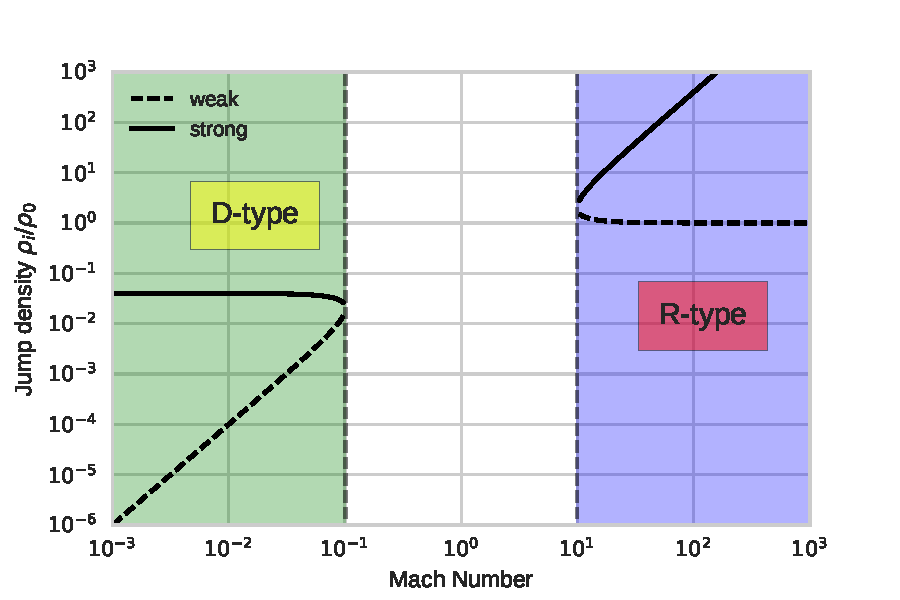
\includegraphics[width=0.5\linewidth]{./Figures/IF-types} &
    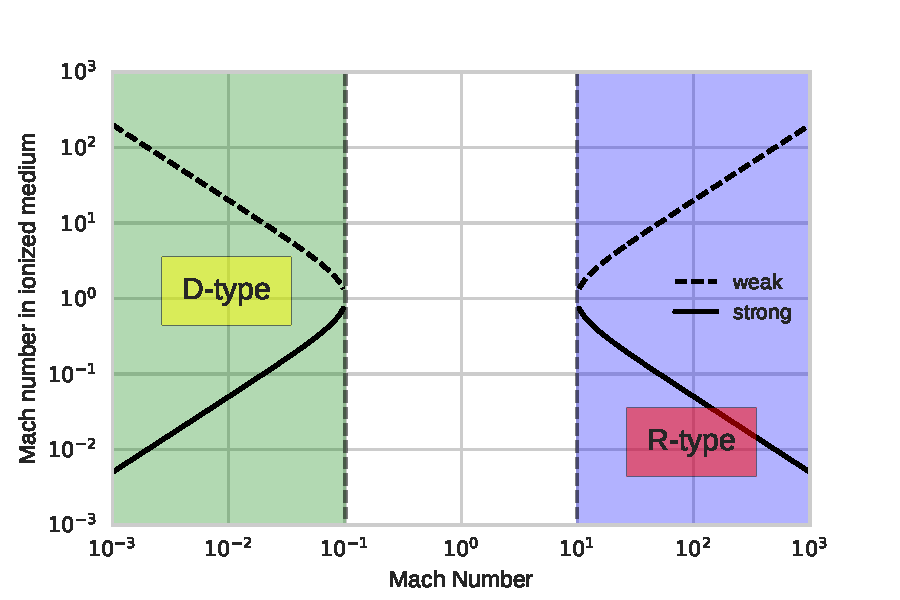
\includegraphics[width=0.5\linewidth]{./Figures/IF-vel-jump}
  \end{tabular}
  \caption{Soluciones para el salto en (a) densidad y (b) velocidad de un frente de ionización. La línea punteada representa la solución a la ecuación (\ref{eq:IF-jump-density})cuando se utiliza el signo negativo, mientras que la línea contínua a la solución con signo positivo. En la región sombreada en verde se muestran los frentes tipo D y en la región azul los frentes tipo R. Los frentes tipo D crítico y R crítico ocurren donde se intersectan las soluciones con las líneas punteadas verticales.}
  \label{fig:IF-jump}
\end{figure}
Por otro lado, el salto en velocidad lo podemos derivar combinando las ecuaciones (\ref{eq:jump-1}, \ref{eq:IF-jump-density}). El resultado se muestra en la figura \ref{fig:IF-jump}b. En el caso de los frentes R crítico y D crítico, la velocidad del gas en el medio ionizado es igual a la velocidad del sonido.

\chapter[Radio de Curvatura]{Derivación Matemática del Radio de Curvatura}
\label{app:math-curvature-radius}
\thispagestyle{empty}
\section{Caso General}
Tomamos una curva genérica $\vec{\sigma}(t) \equiv x(t) \hat{x} + y(t) \hat{y}$ continua y suave para todo valor de $t$ real y finito. Sus derivadas se denotan como $\vec{\sigma}'(t)$ y $\vec{\sigma}''(t)$. Su longitud de arco está dada por:

\begin{align}
  s(t) = \int^t_0 \norm{\vec{\sigma}'(t')}~dt' \label{eq:arc-length}
\end{align}

Reparametrizamos la trayectoria $\vec{\sigma}(t)$ con la longitud de arco y diferenciando respecto a ésta obtenemos lo siguiente:

\begin{align}
  \frac{d\vec{\sigma}}{ds} = \frac{\vec{\sigma}'(t)}{\norm{\vec{\sigma}'(t)}} \equiv \vec{T}(s)
\end{align}

Esta última expresión se logró diferenciando la ecuación (\ref{eq:arc-length}) y aplicando la regla de la cadena al diferenciar $\frac{d\vec{\sigma}}{ds}$. $\vec{T}(s)$ es el vector tangente a la trayectoria $\vec{\sigma}(s)$.

La curvatura $\kappa$ se define como la magnitud de la derivada del vector tangente respecto a la longitud de arco, o bien, como la segunda derivada de la trayectoria $\vec{\sigma}(s)$:

\begin{align}
  \kappa \equiv \norm{\vec{T}'(s)} = \norm{\vec{\sigma}''(s)} 
\end{align}

El radio de curvatura se define como el radio de un círculo que ajusta localmente a la trayectoria, y se calcula como el inverso
multiplicativo de la curvatura:

\begin{align}
  R_c = \frac{1}{\kappa}
\end{align}

Aplicando la regla de la cadena encontramos la siguiente expresión para la curvatura:

\begin{align}
  \kappa = \norm{\frac{\vec{\sigma}''(t)}{\norm{\vec{\sigma}'(t)}^2} - \frac{\vec{\sigma}'(t)}{\norm{\vec{\sigma}'(t)}^4}
  \vec{\sigma}'(t)\cdot\vec{\sigma}''(t)} \label{eq:curvature}
\end{align}

Escribimos las componentes de las derivadas de $\vec{\sigma}(t)$ para calcular los factores que intervienen en la
ecuación (\ref{eq:curvature}):

\begin{align} 
  \vec{\sigma}'(t) &= \dot{x}\hat{x} + \dot{y} \hat{y} \\
  \vec{\sigma}''(t) &= \ddot{x} \hat{x} +  \ddot{y} \hat{y} \\
  \implies \vec{\sigma}'(t)\cdot\vec{\sigma}''(t) &= \dot{x}\ddot{x} + \dot{y}\ddot{y}
\end{align}

De esta forma, calculamos la curvatura como sigue:

\begin{align}
  \kappa &= \left[\left(\frac{\ddot{x}}{\norm{\vec{\sigma}'}^2} - \frac{\dot{x}(\dot{x}\ddot{x} + \dot{y}\ddot{y})}{\norm{\vec{\sigma}'}^4}\right)^2
  + \left(\frac{\ddot{y}}{\norm{\vec{\sigma}'}^2} - \frac{\dot{y}(\dot{x}\ddot{x} + \dot{y}\ddot{y})}{\norm{\vec{\sigma}'}^4} 
\right)^2\right]^{1/2} \\
\begin{split}
 \kappa  &= \norm{\vec{\sigma}'}^{-2}\left[\left(\ddot{x}(\dot{x}^2 + \dot{y}^2) - \dot{x}(\dot{x}\ddot{x} + \dot{y}\ddot{y})\right)^2\\
    & + \left(\ddot{y}(\dot{x}^2 + \dot{y}^2) - \dot{y}(\dot{x}\ddot{x} + \dot{y}\ddot{y})\right)^2 \right]^{1/2}
\end{split}\\
 \kappa  &= \norm{\vec{\sigma}'}^{-2}\left[\left(\ddot{x}\dot{y}^2 - \dot{x}\dot{y}\ddot{y}\right)^2 +
   \left(\ddot{y}\dot{x}^2 - \dot{y}\dot{x}\ddot{x}\right)^2 \right]^{1/2} \\
 \kappa  &=\norm{\vec{\sigma}'}^{-3}\left[\ddot{x}^2\dot{y}^2 + \ddot{y}^2\dot{x}^2 - 2\ddot{x}\ddot{y}\dot{x}\dot{y}\right]^{1/2} \\
\kappa &= \frac{\left|\ddot{x}\dot{y} - \ddot{y}\dot{x}\right|}{\left(\dot{x}^2+\dot{y}^2\right)^{3/2}} 
\end{align}

Utilizando coordenadas polares, y utlizando el ángulo polar $\theta$ como parámetro, la expresión para el radio de curvatura queda como sigue:

\begin{align}
R_c = \frac{\left(R^2 + R^2_\theta\right)^{3/2}}{\left|R^2 + 2R_\theta -RR_{\theta\theta}\right|}\label{eq:Rc-generic}
\end{align}

Donde $R_\theta \equiv \frac{dR}{d\theta}$ y $R_{\theta\theta} \equiv \frac{d^2R}{d\theta^2}$.

Evaluando (\ref{eq:Rc-generic}) en el ápex $(\theta = 0)$ encontramos que $R_{\theta, 0} = 0$ por ser el mínimo de $R(\theta)$ y podemos quitar las barras de valor absoluto porque el denominador resultante siempre es positivo por la misma razón. Por tanto recuperamos la ecuación (\ref{eq:generic-Rc}):

\begin{align}
R_c = \frac{R_0^2}{R- R_{\theta\theta, 0}}\label{eq:Rc-apex}
\end{align}

\section[Polinomio Grado $2n$]{Radio de curvatura para un polinomio de grado $2n$}
\label{app:curvature-radius-poly}

Dado que es de nuestro interés calcular el radio de curvatura del choque en el eje de simetría
$(\theta=0)$, debido a que es analíticamente más fácil de calcular, y a su vez es medible
observacionalmente ajustando un círculo a una serie de mediciones de la posición del choque (sección ).
Entonces, hacemos una aproximación para la función $R(\theta)$ que nos da la forma del choque
mediante un polinomio par de grado $2n$ de la siguiente forma:

\begin{align}
R(\theta) \simeq R_0\left(1 + R_{\theta \theta, 0}\theta^2 + \mathcal{O}(\theta^4)\right)
\end{align}

De esta forma calculamos las derivadas de $R(\theta)$:

\begin{align}
  \dot{R}(\theta) &\simeq R_0\theta\left(2R_{\theta \theta, 0} + \mathcal{O}(\theta^2)\right) \\
  \ddot{R}(\theta) &\simeq R_0\left(2R_{\theta \theta, 0} + \mathcal{O}(\theta^2)\right)
\end{align}

Evaluando en $\theta = 0$ obtenemos los siguiente:

\begin{align}
  R(0) &= R_0 \\
  \dot{R}(0) &= 0 \\
  \ddot{R}(0) &= 2R_{\theta \theta, 0} R_0 \\
  \implies \omega(0) &= 0 \\
  \dot{\omega}(0) &\equiv \frac{\ddot{R}(0)}{R(0)} - \left(\frac{\dot{R}(0)}{R(0)}\right)^2 = 2R_{\theta \theta, 0}
\end{align}

Sustituyendo en la ecuación (\ref{eq:Rc-generic}) obtenemos la planitud en el ápex:

\begin{align}
  \Pi = \frac{1}{\left|1 - 2R_{\theta \theta, 0}\right|}\label{eq:Rc-nose}
\end{align}

Por esto en el apéndice \ref{app:derivation-radii} para encontrar el radio de curvatura nos enfocamos en encontrar
el coeficiente de segundo orden en la expansión en serie de $R(\theta)$.

\chapter[Matrices de Rotación]{Matrices de Rotación y Proyección en el Plano del Cielo.}
\label{app:matrix}
\thispagestyle{empty}
La transformación del sistema de referencia del objeto (no primado) al sistema de referencia del plano del cielo (primado), se realiza mediante una rotación respecto al eje $y$ por un ángulo $i$. Dicha rotación es descrita por la matriz de rotación $\mathbf{A}_y(i)$:

\begin{align}
  \mathbf{A}_y(i) = \left(
  \begin{array}{ccc}
    \cos i & 0 & -\sin i \\
    0      & 1 & 0       \\
    \sin i & 0 & \cos i
  \end{array}\right)
\end{align}

A su vez se pueden obtener con esta matriz los vectores unitarios del sistema de referencia primado en términos de los vectores unitarios del sistema de referencia no primado:

\begin{align}
  \hat{x}' = \mathbf{A}_y(-i)\left(
  \begin{array}{c}
    1 \\ 0 \\ 0
  \end{array}\right)\\
  \hat{y}' = \mathbf{A}_y(-i)\left(
  \begin{array}{c}
    0 \\ 1 \\ 0
  \end{array} \right)\\
  \hat{z}' = \mathbf{A}_y(-i)\left(
  \begin{array}{c}
    0 \\ 0 \\ 1
  \end{array}\right) \label{eq:y-matrix}
\end{align}

Es de notarse que en este caso el signo de $i$ está invertido debido a que actualmente la matriz de rotación $\mathbf{A}_y(i)$ realiza una rotación en favor de las manecillas del reloj, mientras que convencionalmente se utiliza el signo positivo del ángulo de rotación para rotaciones en contra de las manecillas del reloj \citep{Bronson}.

Por otro lado, como estamos considerando choques con geometría cilíndrica, entonces todos los ángulos azimutales $\phi$ son equivalentes. Entonces, por simplicidad, podemos trabajar con curvas bidimensionales en plano $xy~(z=0)$, donde su forma tridimensional es una superficie de revolución de éstas alrededor del eje $x$ y se puede encontrar mediante la matriz de rotación:

\begin{align}
  \mathbf{A}_x(\phi) = \left(
  \begin{array}{ccc}
    1 & 0        & 0         \\
    0 & \cos\phi & -\sin\phi \\
    0 & \sin\phi & \cos\phi
  \end{array}
  \right) \label{eq:x-matrix}
\end{align}

Donde $\phi$ toma valores en el intervalo $[0, 2\pi]$

\chapter[Derivación de Radios Característicos]{Derivación paso a paso de los Radios Característicos en el Modelo de Capa Delgada}
\label{app:derivation-radii}
\thispagestyle{empty}
\section{$R_0$}
Podemos determinar el radio característico $R_0$ a partir de la condición de que el choque es estacionario. En este caso,
los momentos de los dos vientos son iguales en la posición del choque. Por tanto, utilizando la ecuación de momento en $\theta=0$
obtenemos lo siguiente:

\begin{align}
  \rho_{ws} v^2_w &= \rho_{ws1} v^2_{w1}
\end{align}
Donde $\rho_{ws}$ y $\rho_{ws1}$ son las densidades de los dos vientos en la posición del choque. Por otro lado, como la tasa de pérdida
de masa es constante para un ángulo $\theta$ dado, entonces podemos hacer lo siguiente:

\begin{align}
  \frac{\dot{M}^0_w}{4\pi R_0^2 v_w}v^2_w &= \frac{\dot{M}^0_{w1}}{4\pi\left(D-R_0\right)^2v_{w1}}v^2_{w1} \label{eq:momento-R0-uf}
\end{align}
En esta última ecuación hemos sustituído $\dot{M}^0_w = 4\pi R_0^2 v_w \rho_{ws}$ y \\
$\dot{M}^0_{w1} = 4\pi \left(D - R_0\right)^2 v_{w1} \rho_{ws1}$.

Reduciendo la ecuación (\ref{eq:momento-R0-uf}) encontramos una expresión para $R_0$:

\begin{align}
  \frac{R_0}{D} = \frac{\beta^{1/2}}{1+\beta^{1/2}}
\end{align}

\section[Alatud]{Alatud de Choques tipo Cantoides y Ancantoides}
\label{app:alatude-derivation}
$R_{90}$ puede determinarse a partir de evaluar las ecuaciones (\ref{eq:R-geometric}) y (\ref{eq:th1-th}) en $\theta=\frac{\pi}{2}$
como sigue:

\begin{align}
  \frac{R_{90}}{D} &= \tan\theta_{1,90} \\
  \theta_{1,90}\cot\theta_{1,90} -1 &=  - \frac{2\beta}{k+2}
\end{align}

Donde $\theta_{1,90} = \theta_1\left(\frac{\pi}{2}\right)$. Introducimos un nuevo parámetro $\xi \equiv \frac{2}{k+2}$ de modo que
combinando las dos ecuaciones anteriores obtenemos lo siguiente:

\begin{align}
  \frac{R_{90}}{D} = \tan\theta_{1,90} = \frac{\theta_{1,90}}{1-\xi\beta} \label{eq:r90-incomplete}
\end{align}

Hacemos una expansión en serie para el lado izquierdo de la ecuación y reducimos:

\begin{align}
  \theta^2_{1,90}\left(1 + \frac{\theta^2_{1,90}}{15}\right) \simeq 3\beta\xi
\end{align}
Tomamos la solución a primer orden $\theta_{1,90} = 3\beta\xi$,  sustituímos este valor en el término correctivo y resolvemos para
$\theta_{1,90}$:

\begin{align}
  \theta_{1,90} = \left(\frac{3\xi\beta}{1+\frac{1}{5}\xi\beta}\right)^{1/2} \label{eq:th190}
\end{align}

Finalmente sustituímos (\ref{eq:th190}) en (\ref{eq:r90-incomplete}) para obtener $R_{90}$:
\begin{align}
  \frac{R_{90}}{D} &= \frac{\left(3\xi\beta\right)^{1/2}}{\left(1+\frac{1}{5}\xi\beta\right)^{1/2}\left(1-\xi\beta\right)} \\
  \Lambda &= \frac{\left(3\xi\right)^{1/2}\left(1+\beta^{1/2}\right)}
                   {\left(1+\frac{1}{5}\xi\beta\right)^{1/2}\left(1-\xi\beta\right)} 
\end{align}

\section[Planitud]{Planitud de choques tipo Cantoides y Ancantoides}

Siendo que el choque de proa en nuestro modelo genérico es simétrico, entonces la forma $R(\theta)$ debe ser una función par,
por tanto podemos hacer la siguiente expansión en serie:

\begin{align}
  R(\theta) \simeq R_0 + \frac{1}{2}R_{\theta\theta, 0}\theta^2 + \mathcal{O}(\theta^4)
\end{align}

De esta forma la planitud del choque en el ápex queda como sigue (ver apéndice \ref{app:math-curvature-radius}):
\begin{align}
  \Pi = \left(1 - 2\frac{R_{\theta \theta, 0}}{R_0}\right)^{-1}
\end{align}

Para encontrar el coeficiente de segundo orden $R_{\theta \theta, 0}$ hacemos una expansión en serie de las ecuaciones (\ref{eq:th1-th}) y
(\ref{eq:R-geometric}) para ángulos pequeños, mostrando a continuación la expansión de cada término para al final hacer la
reducción algebraica:

\begin{align}
  \theta_1\cot\theta_1 -1 &\simeq -\frac{\theta^2_1}{3}\left(1 + \frac{\theta^2_1}{15}\right) \\
  \cos^k\theta &\simeq \left(1 - \frac{\theta^2}{2}\right)^k \simeq \left(1 - \frac{k\theta^2}{2}\right) \\
  \sin^2\theta &\simeq \theta^2\left(1 - \frac{\theta^2}{6}\right)^2 \simeq \theta^2\left(1 - \frac{\theta^2}{3}\right)\\
  \implies \cos^k\theta\sin^2\theta &\simeq \theta^2\left[1 - \left(\frac{1}{3} + \frac{k}{2}\right)\theta^2\right] \\
  \implies I_k(\theta) &\simeq \frac{\theta^3}{3}\left[1 - \frac{1}{10}\left(3k + 2\right)\theta^2\right] \\
  \cot\theta &\simeq \theta^{-1}\left(1 - \frac{\theta^2}{3}\right) \\
  \implies 2\beta I_k(\theta)\cot\theta &\simeq \frac{2}{3}\beta\theta^2\left[1 - \frac{1}{30}\left(9k + 16\right)\theta^2\right] \\
  -\frac{2\beta}{k+2}\left(1 - \cos^{k+2}\theta\right) &\simeq \beta\theta^2\left[1 - \frac{1}{12}\left(3k+4\right)\right]
\end{align}

Sustituyendo las expansiones anteriores en (\ref{eq:th1-th}) obtenemos lo siguiente:
\begin{align}
  \theta^2_1\left(1 + \frac{\theta^2_1}{15}\right) \simeq \beta\theta^2\left[1 + \frac{1}{60}\left(4 - 9k\right)\theta^2\right]
  \label{eq:th1-th-approx}
\end{align}

La solución a primer orden (ignorando el término cuártico) es $\theta^2_ 1 \simeq \beta\theta^2$. Sustituímos esta solución en el
término correctivo y resolvemos para $\theta^2_1$:

\begin{align}
  \theta^2_1 &\simeq \beta\theta^2\left[1 + \frac{1}{60}\left(4 - 9k\right)\theta^2\right]\left(1 + \frac{\beta\theta^2}{15}\right)^{-1} \\
  \theta^2_1 &\simeq \beta\theta^2\left[1 + \frac{1}{60}\left(4 - 9k\right)\theta^2\right]\left(1 - \frac{\beta\theta^2}{15}\right) \\
  \implies \theta^2_1 &\simeq \beta\theta^2\left(1 + C_{k\beta}\theta^2\right) \\
  \mathrm{Donde:\quad}C_{k\beta} &= \left(\frac{1}{15} - \frac{3k}{20} - \frac{\beta}{15}\right)
\end{align}

Utilizamos esta solución para $\theta_1$ en la ecuación (\ref{eq:R-geometric}), ignorando términos de orden superior al cuártico
dentro de los corchetes:

\begin{align}
  \theta_1 &\simeq \beta^{1/2}\theta\left(1 + C_{k\beta}\theta^2\right)^{1/2} \\
  \implies \theta + \theta_1 &\simeq \theta\left[1 + \beta^{1/2}\left(1 + \frac{C_{k\beta}}{2}\theta^2\right)\right]\\ 
  \sin\theta_1 &\simeq \theta_1\left(1 - \frac{\theta^2_1}{6}\right) \\
  &\simeq \beta^{1/2}\theta\left(1 + \frac{C_{k\beta}}{2}\theta^2\right)\left[1 - \frac{\beta\theta^2\left(1 + C_{k\beta}\theta^2\right)}{6}\right]\\
  \implies \sin\theta_1 &\simeq \beta^{1/2}\theta\left[1 + \left(\frac{C_{k\beta}}{2}- \frac{\beta}{6}\right)\theta^2\right]
\end{align}
\begin{align}
  \sin\left(\theta + \theta_1 \right) &\simeq \left(\theta + \theta_1\right)\left[1 - \frac{\left(\theta + \theta_1\right)^2}{6}\right] \\
           &\simeq \theta\left[1 + \beta^{1/2}\left(1 + \frac{C_{k\beta}}{2}\theta^2\right)\right] \left[1 - \frac{\theta^2\left(1 + \beta^{1/2}
             \left(1 + \frac{C_{k\beta}}{2}\theta^2\right)\right)^2}{6}\right] \\
           &\simeq \theta\left(1 + \beta^{1/2}\right)\left[1 + \left(\frac{\beta^{1/2}C_{k\beta}}{2\left(1 + \beta^{1/2}\right)} - \frac{1}{6}\left(1 + \beta^{1/2}\right)^2
             \theta^2\right)\right]\\
\begin{split}
  \implies \frac{R}{D} &\simeq \frac{\beta^{1/2}}{1 + \beta^{1/2}}\left[1 + \left(\frac{C_{k\beta}}{2} - \frac{\beta}{6}\right)\theta^2\right] \\
               & \left[1 + \left(\frac{\beta^{1/2}C_{k\beta}}{2\left(1 + \beta^{1/2}\right)} - \frac{\left(1 + \beta^{1/2}\right)^2}{6}\right)\theta^2\right]^{-1} 
\end{split}\\
  &\simeq R_0 \left[1 + \left(\frac{C_{k\beta}}{2\left(1+\beta^{1/2}\right)} + \frac{1+2\beta^{1/2}}{6}\right)\theta^2\right] 
\end{align}

De esta mostramos que el término de segundo órden que necesitamos en la ecuación (\ref{eq:CRW-Rc}) está dado por:

\begin{align}
  \frac{R_{\theta\theta, 0}}{2} = \frac{C_{k\beta}}{2\left(1+\beta^{1/2}\right)} + \frac{1+2\beta^{1/2}}{6}
\end{align}

que es el resultado mostrado en la ecuación (\ref{eq:2-order})

\section[Planitud Wilkinoides]{Planitud para choques tipo Wilkinoides}
\label{sec:Rc-Wilkin}
Hacemos expansión Taylor hasta cuarto orden de cada uno de los términos de la ecuación (\ref{eq:R-Wilkin})

\begin{align}
  \csc^2\theta &\simeq \theta^{-2}\left(1 - \frac{\theta^2}{6} + \mathcal{O}(\theta^4)\right)^{-2} \simeq
                 \theta^{-2}\left(1 + \frac{\theta^2}{3} + \mathcal{O}(\thta^4)\right) \\
  \theta\cot\theta &\simeq 1 - \frac{\theta^2}{3}\left(1 + \frac{\theta^2}{15} + \mathcal{O}(\theta^4)\right) \\
  \implies 1 -\theta\cot\theta &\simeq \frac{\theta^2}{3}\left(1 + \frac{\theta^2}{15} + \mathcal{O}(\theta^4)\right)
\end{align}

Sustituímos en la ecuación (\ref{eq:R-Wilkin}):

\begin{align}
  R(\theta) &\simeq R_0\left[3\theta^{-2}\left(1 + \frac{\theta^2}{3}+\mathcal{O}(\theta^4)\right)\frac{\theta^2}{15}
  \left(1 + \frac{\theta^2}{15}\right) \right]^{1/2} \\
  \implies R(\theta) &\simeq R_0\left[1 + \frac{2\theta^2}{5} + \mathcal{O}(\theta^4)\right]^{1/2} \\
  \implies R(\theta) &\simeq R_0\left[1 + \frac{\theta^2}{5} + \mathcal{O}(\theta^4)\right]
\end{align}

De esta forma mostramos que el coeficiente de segundo orden en este caso es $R_{\theta \theta, 0} = \frac{1}{5}$. Por lo tanto,
sustituyendo este valor en la ecuación (\ref{eq:Rc-nose}) encontramos que

\begin{align}
  \Pi = \frac{5}{3}
\end{align}

\chapter{True Versus Apparent Shapes of Bowshocks}
\label{app:article}
\thispagestyle{empty}

Este artículo contiene gran parte de esta Tesis, actualmente publicado en la revista Monthly Notices of the Royal Astronomical Society (MNRAS) en Marzo de 2018 \citep{Tarango-Yong:2018a}. 
\setkeys{pdfpages}{pages=-}
\includepdf{quadrics-bowshock.pdf}